\begin{document}
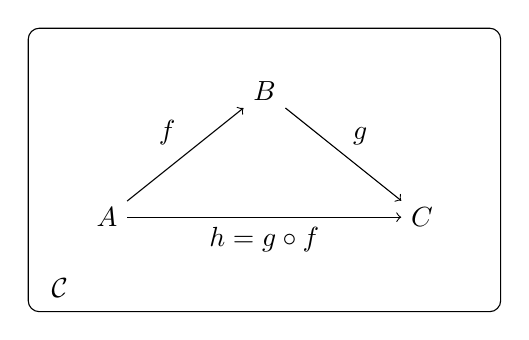
\begin{tikzpicture}
  \draw[rounded corners] (-3,-1.8) rectangle (3,1.8);
  \node at (-2.6,-1.5) {$\mathcal{C}$};
  \node (A) at (-2,-0.6) {$A$};
  \node (B) at (0,1) {$B$};
  \node (C) at (2,-0.6) {$C$};
  \draw[->] (A) -- node[above left] {$f$} (B);
  \draw[->] (B) -- node[above right] {$g$} (C);
  \draw[->] (A) -- node[below] {$h = g \circ f$} (C);
\end{tikzpicture}
\end{document}
